\chapter{Implementação de uma solução}

\section{A Implementação}

Este capitulo demonstrará a implementação de certas funcionalidades baseada na arquitetura apresentada anteriormente. Estas irão modulos de frontend, backend e as pipelines de deployment necessárias. 

\subsection{Frontend}

\subsection{Backend}

\subsection{Deployments}

Como foi explicado anteriormente, um dos requisitos definidos  era a criação de um ambiente de \textit{CI/CD} que permitisse simplicar o processo de desenvolvimento, facilitando a disponibilização de novas versões.

A plataforma Azure disponbiliza a funcionalidade \textit{Pipelines}. Com o recurso à linguagem YAML, esta permite definir os trabalhos que os "agentes" definidos pelo utilizador

Finalmente, utilizando a ferramenta Docker é possível é possivél "empacotar" o código numa só unidade que funciona de forma igual em diferentes máquinas. Esta funcionalidade será feita numa màquina Linux Ubuntu 24.04.2. 

\subsubsection{Definição dos agentes}

No contexto do Azure Pipelines um agente (em inglês, \textit{Agent}) é a maquiná indica ao Azure Pipelines que executará os trabalhos pedidos, como por exemplo compilar o projeto. 

Neste caso iremos indicar ao Azure Pipelines para que utilize a nossa máquina como um agente. O agente irá executar dentro de um \textit{container Docker}.

A Microsoft oferece ferramentas para ajudar neste processo \cite{run-a-self-hosted-agent-in-docker}. O script que estabelece a relação entre os agentes e os serviços Azure, tal como o Dockerfile necessário para a compilção do Docker poderá ser encontrado no anexos \ref{app:pipeline-start.sh} e \ref{app:dockerfile-pipeline-agent} respetivamente.

Após a criação do agente basta iniciar o \textit{container Docker}, tendo em atenção à indicação das variaveis de ambiente necessárias. A figura \ref{fig:start-docker-agent} demonstra isso mesmo, com censura a qualquer informação sensivel à organização.

\begin{figure}
    

\begin{lstlisting}
    sudo docker run -d 
        -e AZP_URL="https://dev.azure.com/blended4future2025" 
        -e AZP_TOKEN="******" 
        -e AZP_POOL="*******" 
        -e AZP_AGENT_NAME="*****" 
        --name "azp-agent-linux" 
        devops-agent:linux
\end{lstlisting}


\caption{Script de inicialização do Container Docker para o agente do Azure Pipelines}
\label{fig:start-docker-agent}

\end{figure}

Logo após, é possivel ver o agente disponível no Azure DevOps (Figura \ref{fig:agent-devops}). 

\begin{figure}
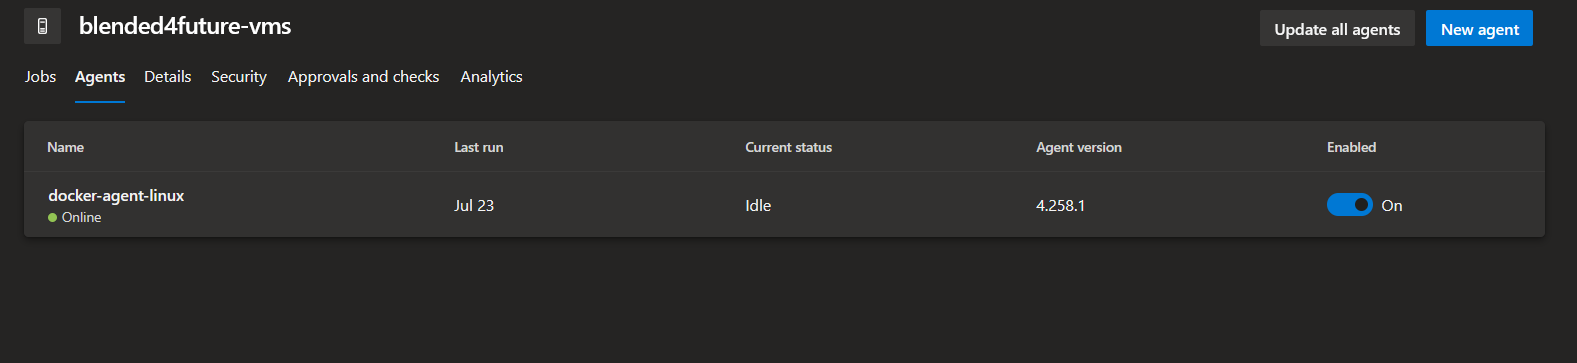
\includegraphics[width=\linewidth]{capitulos/cap4-implementacao/assets/devops-agent.png}
\caption{Agente disponbilizado no Azure DevOps}
\label{fig:agent-devops}
\end{figure}

\subsubsection{Trabalhos da pipeline}

7

\section{Testes}

\subsection{Testes Unitários}

\subsection{Testes de Implementação}

\section{Avaliação da solução}